\documentclass[../_main/handlingar.tex]{subfiles}

\begin{document}
\proposition{Renovering och ombyggnad av HK och BD}

Så som det ser ut idag används inte större delar av BD, rummet används framför allt till att hänga av sig kläder och värma mat under lunchen. Om man sen kollar på HK så används detta rummet flitigt men eftersom rummet är så litet som det är kan max 2-3 personer sitta och arbeta samtdigt. Detta försvårar arbetet för alla som ska utföra admistrativt arbete för Sektionen men framförallt för styrelsen, ett större rum hade gjort att fler personer kunnat jobba parallellt. Vi skulle därför vilja ändra proportionerna på rummen till ungefär det motsatta från nuläget samt renovera upp rummen och införskaffa nya inventarier.

Bilden nedan är ett förslag på hur rummen kan utformas men inte begränsat till det.

\begin{center}
    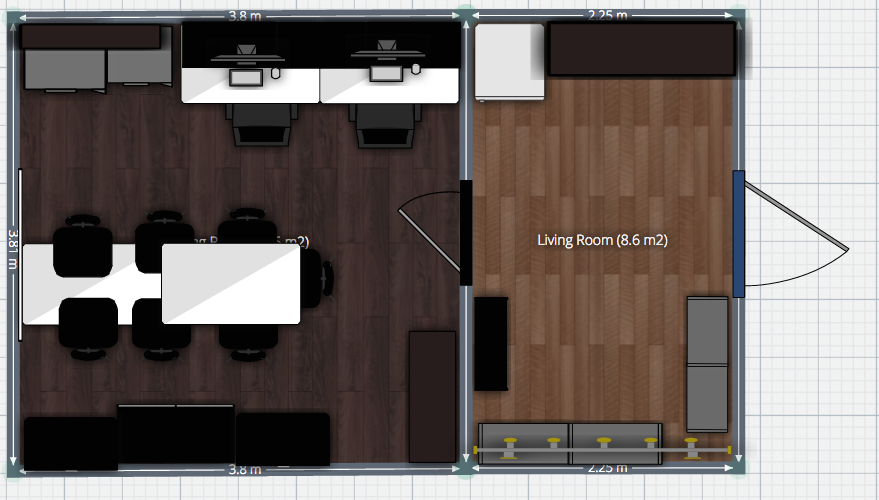
\includegraphics[width=14cm]{hkbla.png}
\end{center}

\newpage

Därför yrkar vi på
\begin{attsatser}
    \att flytta väggen i rummet så BD blir 1/3 och HK blir 2/3 av den totala ytan.
    %\att ändra om proportionerna på rummen så blådörren motsvarar 1/3 och HK motsvarar 2/3 av hela rummet.
    \att en budget på 30000kr avsätts till projektet. Budgeten ska täcka renoverings/ombyggnadskostnaderna, inköpskostnader av möblemang samt mat/tack-kostnader.
    \att kostnaden belastar utrustningsfonden.
    \att de som arbetar ska tackas med mat när det jobbar samt matbiljetter 40kr/st som som kan lösas in under hösten mot mat eller dylikt i LED eller klägg på gille.
    \att detta läggs på beslutsuppföljningen till HT/16 där sittande styrelsen står som ansvarig.
    \att projektet ska utföras i sommar och ska vara klart innan nollningens början.
\end{attsatser}

\begin{signatures}{2}
    \ist
    \signature{Anders Nilsson}{Förvaltningschef}
    \signature{Fredrik Peterson}{Ordförande}
\end{signatures}

\end{document}
